

\chapter{Introducción}
El objetivo de esta tesis es encontrar soluciones periódicas a ecuaciones diferenciales con medidas o MDE\index{MDE}, las cuales se pueden definir de manera general como 
	\begin{equation*}
	\left\lbrace \begin{array}{l} \label{eq:problema A}
		d\varphi=F(t,\varphi(t))\;d \mu\\
		\varphi(0)-\varphi(T)=0,
	\end{array}\right. \tag{${MDE}$}
\end{equation*}
donde $F:[0,T]\times\rr^n\to\rr^{n\times m}$ es una función con valores matriciales, \highlight[comment={Diría más bien: es una medida vectorail con valores en $\mathbb{R}^m$}]{$\mu$ es un vector  $\rr^m$ de medidas}, $\varphi:[0,T]\to \rr^n$ es una función de variación acotada  y $d\varphi$ es \replaced{la medida vectorial}{el vector de medidas} de Lebesgue-Stieltjes asociado a $\varphi$.

Las MDE intervienen en campos de las matemáticas y las ciencias, como por ejemplo sistemas mecanicos ( ver \cite{Brogliato} y \cite{ALeonov}), entre otros.\comment{¿Desarrollamos un poco más?}


Un caso particular interesante, donde intervienen MDE, son los problemas impulsivos, ver \cite{Bainov} y \cite{Lakshmikan}. Por ejemplo, en los sistemas mecánicos se puede pensar que el impacto entre dos cuerpos es un fenómeno de muy corta duración, que implica un cambio brusco en la dinámica de los cuerpos. Es por eso que se suele representar los impactos como fuerzas muy grandes que actúan en un tiempo infinitamente corto. Supongamos que durante el impacto o colisión actúa una fuerza $F$ y que este ocurre en un intervalo $[t_0,t_0+\Delta t]$, entonces el cambio en la cantidad de movimiento es igual al impulso que genera la fuerza \index{impulso} \cite{Serway}, 
$$I=\Delta p=\int_{t_0}^{t_0+\Delta t}f(s)ds.\textrm{\todo{Es $f$ o $F$?}}$$
Si suponemos que la fuerza actúa en un intervalo muy chico, es decir que es instantánea entonces el impulso sera
    \begin{equation*}
        I=\lim_{\Delta t \to 0}\int_{t_0}^{t_0+\Delta t}F(s) ds. 
    \end{equation*}
Para que el impulso $I$ sea distinto de cero, $F(\cdot)$ debe tomar valores infinitos ya que la medida de Lebesgue del intervalo tiende a cero. Por eso es conveniente tomar a la fuerza como una medida concentrada en el tiempo $t_0$ y de magnitud $I$, es decir \highlight[comment={decir que  cosa es $\delta$}]{$F(t)=I\delta_{t_0}$}, a este tipo de fuerza se la  denomina fuerza impulsiva\index{fuerza impulsiva}.

\begin{example} \label{ejemplo1}
    Supongamos que un cuerpo de masa $m$ se mueve con velocidad constante sobre una recta, y se somete a impulsos $I_k$ en los instantes $t_k$. Como el impulso es el cambio en la cantidad de movimiento (\cite{Serway}) entonces $I_k=mv(t_k^+)-mv(t_k^-)$. Podemos decir que si el movimiento del cuerpo está dado por la función $x(t)$, entonces cumple la siguiente ecuación 
    \begin{equation}
	\left\lbrace \begin{array}{lll} 
		\label{eq:imp}
        x''(t)=0 & \text{si }& t\neq t_k,\\
		x'(t_k^+)-x'(t_k^-)=\dfrac{I_k} {m} & \text{ para }& k=1,..,r.\tag{${PI}$}
	\end{array}\right. 
\end{equation}
Si ahora consideramos que la fuerza es impulsiva $F(t)=\displaystyle\sum_{k=1}^r I_k\delta_{t_k}$ entonces puedo escribir el problema impulsivo \ref{eq:imp} como \added{una} \ref{eq:problema A}
$$x''(t)=\sum_{k=1}^r\dfrac{I_k}{m}\delta_{t_k}$$
\end{example}

\todo{Me parece que el lector quizás no entienda cual es la relación de la ecuación anterior con la ecuación impulsiva puesta de ejemplo. Podés referirte brevemente a que es una solución.  Poner $dx'$ en lugar de $x''$ y a grandes rasgos decir porque una solución de la ecuación con medidas es solución del problema impulsivo}



%\begin{example}
%    \begin{equation*}
%	\left\lbrace \begin{array}{lcr} 
%		x'=1+x^2,\\
%        x(0)=0\\
%		\Delta x(t_k)=-1 &t_k=\frac{k\pi}{4}&k=1,2,....
%	\end{array}\right. 
%\end{equation*}
%Si notamos $d\lambda$ a la medida de Lebesgue \index[Simbolo]{$d\lambda$}, el problema anterior se puede expresar como una MDE de la siguiente manera
%\begin{equation*}
%	\left\lbrace \begin{array}{lcr} 
%		x'=1+x^2 \;d\lambda-\displaystyle\sum_{k=1}^{\infty}d\delta_{t_k}(t),\\
%        x(0)=0.\\
	%	\end{array}\right. 
%\end{equation*}
%La solución es $x(t)=\tan(t-\frac{k\pi}{4})$ donde $\frac{k\pi}{4}\leq %t <\frac{(k+1)\pi}{4}$, y tiene período $\pi/4$.
%\begin{figure}[h!]
%    \centering
%    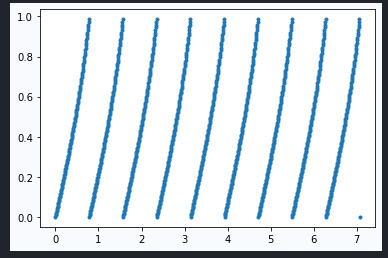
\includegraphics[width=0.7\linewidth]{img.ejem1.png}
%    \caption{}
%    \label{fig:ejemple1}
%\end{figure}



%\end{example}
Las ecuaciones impulsivas se pueden generalizar para casos donde actúen fuerzas no impulsivas $f(t,x)$ y/o donde se aplique una cantidad infinita de impulso. Un caso general se puede ver en \cite{Bainov}, el cual es

	\begin{equation*}
		\left\lbrace \begin{array}{l}
			x''=f(t,x(t)) \; \text{si }\; t\neq t_k\\
			 x'(t_k^+)-x'(t_k^-)=I_k \; \text{ donde }\; k=1,2,....,
		\end{array}\right. 
	\end{equation*}
donde, como vimos en el ejemplo, se pude pensar a los impulsos como suma, de deltas de Dirac concentradas en $t_k$ y la medida de Lebesgue $d\lambda$.\index[Simbolo]{$d\lambda$}  
\reversemarginpar
$$x''=f(t,x(t)) d\lambda +\sum_{k=1}^{\infty}\dfrac{I_k}{m}\;d\delta_{t_k}\textrm{\todo{\small falta o sobra un $m$ en algún lugar}}$$

Para resolver ecuaciones como \ref{eq:problema A}, usaremos una metodología inspirada en el libro de Pablo Amster \cite{Amster}, sobretodo en la sección 1.3. Allí utiliza el método Shooting para hallar soluciones al problemas de contorno periódico 

	\begin{equation*}
		\left\lbrace \begin{array}{l}
			u'=f(t,u(t))\\
			u(0)-u(T)=0,
		\end{array}\right. 
	\end{equation*}
donde $f$ es una función continua y Lipschitz en la segunda variable $u\in\rr^2$.  La idea que propone Pablo Amster es buscar una solución $u_\alpha$ al problema de valores iniciales 
	\begin{equation*}
	\left\lbrace \begin{array}{lcl}
		u'&=&f(t,u(t))\\
		u(0)&=&\alpha,
	\end{array}\right. 
\end{equation*}
y buscar un valor de $\alpha\in\rr^2$ tal que $u_\lambda(T)=\alpha$. No es otra cosa que un punto fijo \replaced{del}{dell} operador \deleted{(operador} de Poíncare\index{operador de Poíncare}\deleted{)} $P:\rr^2\to \rr^2$, definido como $P(\alpha)=u_\alpha(T)$. \replaced{Bajo ciertas condiciones, aplicando}{ Aplicando} el Teorema de Brouwer \cite{Amster} al operador \added{$P$} podemos asegurar la existencia de la solución al problema periódico. 

En el capitulo 2 haremos una breve introducción a la medida de Lebesgue-Stieltjes y sus propiedades.  En la sección 3.1 vamos a ver como transformar el problema \eqref{eq:problema A} con medidas vectoriales a uno donde intervenga una sola medida positiva, en la sección 3.2 veremos las condiciones para la existencia de soluciones al problema de valores iniciales y su continuación a intervalos máximos. En la sección 3.3 enunciaremos y demostraremos una versión del teorema de Gronwall que hemos obtenidos para medidas de Borel. A partir de este teorema demostramos la continuidad del operador de Poíncare y finalmente podremos usar el Teorema Brouwer y  hallaremos un punto fijo para el operador de Poincaré.  \todo{Falta lo que se hace en capítulo 4}
